\documentclass[11pt,a4paper]{report}

% ===================== PACKAGES =====================
\usepackage[utf8]{inputenc}
\usepackage[T1]{fontenc}
\usepackage[french]{babel}
\usepackage[a4paper,left=2.7cm,right=2.5cm,top=2.6cm,bottom=2.6cm]{geometry}
\usepackage{graphicx}
\usepackage{xcolor}
\usepackage{booktabs}
\usepackage{longtable}
\usepackage{array}
\usepackage{caption}
\usepackage{float}
\usepackage{enumitem}
\usepackage{fancyhdr}
\usepackage{titlesec}
\usepackage{tocloft}
\usepackage{listings}
\usepackage{hyperref}
\usepackage{colortbl}
\usepackage{tabularx}
\usepackage{setspace}

% ===================== COULEURS =====================
\definecolor{primaryblue}{HTML}{2E5C8A}
\definecolor{lightblue}{HTML}{EAF2FB}
\definecolor{darkgrey}{HTML}{333333}
\definecolor{okgreen}{HTML}{3C8C3C}
\definecolor{warnorange}{HTML}{B8860B}
\definecolor{errred}{HTML}{A94442}
\definecolor{codebg}{HTML}{F6F8FA}

% ===================== TITRES =====================
\titleformat{\chapter}[display]
  {\normalfont\huge\bfseries\color{primaryblue}}
  {\chaptertitlename\ \thechapter}{16pt}{\Huge}
\titleformat{\section}
  {\normalfont\Large\bfseries\color{primaryblue}}{\thesection}{1em}{}
\titleformat{\subsection}
  {\normalfont\large\bfseries\color{darkgrey}}{\thesubsection}{1em}{}

% ===================== EN-TETES =====================
\pagestyle{fancy}
\fancyhf{}
\renewcommand{\headrulewidth}{0.4pt}
\fancyhead[L]{\small\textit{Agent IA Autonome — AWS Bedrock + LangChain}}
\fancyhead[R]{\small\thepage}
\fancyfoot[C]{\small Smartovate Ltd — Rapport de stage}

% ===================== CODE =====================
\lstdefinestyle{python}{
  backgroundcolor=\color{codebg},
  basicstyle=\ttfamily\footnotesize,
  keywordstyle=\color{primaryblue}\bfseries,
  commentstyle=\color{okgreen}\itshape,
  stringstyle=\color{errred},
  numbers=left, numberstyle=\tiny\color{gray}, numbersep=6pt,
  frame=single, rulecolor=\color{gray!40},
  breaklines=true, breakatwhitespace=true,
  showstringspaces=false, tabsize=4,
  language=Python,
  xleftmargin=1.2em,
}
\lstset{style=python}

% ===================== HYPERREF =====================
\hypersetup{
  colorlinks=true, linkcolor=primaryblue, citecolor=primaryblue,
  urlcolor=primaryblue, pdftitle={Agent IA Autonome avec AWS Bedrock et LangChain},
  pdfauthor={SIMPORE W. Flore}
}

% Boîte "à compléter" pour signaler clairement les captures/schémas manquants
\newcommand{\tocomplete}[1]{%
  \par\noindent\fcolorbox{errred}{errred!8}{%
    \parbox{0.95\linewidth}{\small \textcolor{errred}{\textbf{[À COMPLÉTER PAR L'AUTEUR — capture d'écran non générable automatiquement]}}\\ #1}%
  }\par\vspace{4pt}
}
\newcommand{\genfigure}[1]{%
  \par\noindent\fcolorbox{okgreen}{okgreen!8}{%
    \parbox{0.95\linewidth}{\small \textcolor{okgreen}{\textbf{[Schéma généré automatiquement — fourni avec ce rapport]}}\\ #1}%
  }\par\vspace{4pt}
}

\newcolumntype{Y}{>{\raggedright\arraybackslash}X}

\begin{document}

% ===================== PAGE DE GARDE =====================
\begin{titlepage}
\centering
\vspace*{0.5cm}

{\large
\begin{minipage}[t]{0.48\linewidth}
\textbf{[LOGO DE L'ÉCOLE / UNIVERSITÉ\\ À AJOUTER]}
\end{minipage}
\hfill
\begin{minipage}[t]{0.48\linewidth}
\raggedleft
\textbf{[LOGO SMARTOVATE LTD\\ À AJOUTER]}
\end{minipage}
}\\[2cm]

{\Large \textsc{Rapport de stage}}\\[0.3cm]
{\large Stage de fin d'études — 2 mois (Juillet -- Août 2026)}\\[1.5cm]

\rule{\linewidth}{0.6pt}\\[0.5cm]
{\huge \textbf{Agent IA Autonome avec}}\\[0.2cm]
{\huge \textbf{AWS Bedrock + LangChain}}\\[0.5cm]
\rule{\linewidth}{0.6pt}\\[1.2cm]

{\large Conception, développement et déploiement d'un agent conversationnel\\
autonome de type ReAct, orchestré avec LangGraph, déployé en\\
architecture serverless sur AWS}\\[2cm]

\begin{minipage}{0.45\textwidth}
\textbf{Présenté par :}\\
SIMPORE W. Flore
\end{minipage}
\hfill
\begin{minipage}{0.45\textwidth}
\raggedleft
\textbf{Encadrement :}\\
Maître de stage (Smartovate Ltd) : \textbf{[À COMPLÉTER]}\\
Tuteur académique : \textbf{[À COMPLÉTER]}
\end{minipage}

\vfill

\begin{center}
\textbf{Entreprise d'accueil : Smartovate Ltd}\\
\textbf{[À COMPLÉTER : ville / pays du siège Smartovate]}\\[0.3cm]
Période de stage : 1\textsuperscript{er} juillet -- 25 août 2026\\[0.3cm]
\textbf{[À COMPLÉTER : nom de l'établissement, filière, année académique]}
\end{center}

\vspace{1cm}
\end{titlepage}

\pagenumbering{roman}

% ===================== REMERCIEMENTS =====================
\chapter*{Remerciements}
\addcontentsline{toc}{chapter}{Remerciements}

\tocomplete{Section à personnaliser entièrement : remerciements au maître de stage,
au tuteur académique, à l'équipe Smartovate Ltd, à l'établissement, et à toute
personne ayant contribué à ce stage. Le paragraphe ci-dessous n'est qu'un
squelette à adapter.}

Je tiens à exprimer ma sincère gratitude à l'ensemble de l'équipe de
Smartovate Ltd pour son accueil et son accompagnement tout au long de ce
stage de deux mois. Je remercie tout particulièrement \textbf{[nom du
maître de stage]}, pour sa disponibilité, ses conseils techniques et la
confiance accordée sur ce projet d'agent IA autonome. Je remercie
également \textbf{[nom du tuteur académique]} pour son suivi pédagogique,
ainsi que l'ensemble du corps enseignant de \textbf{[établissement]}
pour la formation qui a rendu ce travail possible.

% ===================== RESUME / ABSTRACT =====================
\chapter*{Résumé}
\addcontentsline{toc}{chapter}{Résumé}

Ce rapport présente le travail réalisé durant un stage de deux mois au
sein de Smartovate Ltd, entreprise de conseil cloud, portant sur la
conception et le développement d'un agent d'intelligence artificielle
autonome. Le projet combine \textbf{AWS Bedrock} (accès managé aux
modèles de fondation Claude et Titan) et \textbf{LangChain / LangGraph}
(orchestration) pour produire un agent suivant le patron
\textbf{ReAct} (Reasoning + Acting), capable de mobiliser cinq outils
(calculatrice, météo, recherche web, recherche documentaire interne,
recherche dans les documents utilisateur), de maintenir une mémoire
conversationnelle court terme et une mémoire sémantique long terme
(OpenSearch Serverless), et d'être interrogé via une interface
Streamlit ou une API HTTP streamée (Server-Sent Events).

Au-delà du développement fonctionnel, une part importante du stage a
consisté à \textbf{fiabiliser} le système existant : mise en place
d'une suite de 161 tests unitaires (logique des cinq outils, cœur de
la boucle ReAct, persistance, limitation de débit), construction d'un
harnais d'évaluation de bout en bout sur 23 scénarios représentatifs
(95,7\,\% de réussite en conditions réelles), correction de plusieurs
anomalies fonctionnelles et de sécurité identifiées en cours de route
(authentification silencieuse défaillante, mémoire sémantique jamais
persistée, permissions IAM trop permissives, secret d'API en clair,
garde-fous de sécurité invisibles côté client, encodage des caractères
corrompu), et durcissement de l'infrastructure définie en AWS CDK
selon le principe du moindre privilège.

\textbf{Mots-clés :} intelligence artificielle générative, agent
autonome, ReAct, LangChain, LangGraph, AWS Bedrock, AWS Lambda,
architecture serverless, retrieval-augmented generation (RAG), tests
logiciels.

\vspace{0.8cm}
\begin{center}\rule{0.4\linewidth}{0.4pt}\end{center}
\vspace{0.5cm}

\begin{otherlanguage}{english}
\chapter*{Abstract}
\addcontentsline{toc}{chapter}{Abstract}

This report presents the work carried out during a two-month
internship at Smartovate Ltd, a cloud consulting company, focused on
designing and developing an autonomous artificial intelligence agent.
The project combines \textbf{AWS Bedrock} (managed access to Claude
and Titan foundation models) with \textbf{LangChain / LangGraph}
(orchestration) to build an agent following the \textbf{ReAct}
(Reasoning + Acting) pattern, capable of using five tools (calculator,
weather, web search, internal knowledge-base retrieval, and
user-document retrieval), maintaining both short-term conversational
memory and long-term semantic memory (OpenSearch Serverless), and
being queried through a Streamlit interface or a streamed HTTP API
(Server-Sent Events).

Beyond feature development, a significant part of the internship
consisted of \textbf{hardening} the existing system: building a suite
of 161 unit tests, an end-to-end evaluation harness covering 23
representative scenarios (95.7\,\% success rate in live conditions),
fixing several functional and security issues discovered along the
way, and tightening the AWS CDK infrastructure to follow the
least-privilege principle.

\textbf{Keywords:} generative artificial intelligence, autonomous
agent, ReAct, LangChain, LangGraph, AWS Bedrock, AWS Lambda,
serverless architecture, retrieval-augmented generation (RAG),
software testing.
\end{otherlanguage}

% ===================== TABLE DES MATIERES =====================
\tableofcontents

% ===================== LISTE DES FIGURES =====================
\listoffigures
\addcontentsline{toc}{chapter}{Table des figures}

% ===================== LISTE DES TABLEAUX =====================
\listoftables
\addcontentsline{toc}{chapter}{Liste des tableaux}

% ===================== ABREVIATIONS =====================
\chapter*{Liste des abréviations}
\addcontentsline{toc}{chapter}{Liste des abréviations}
\begin{tabularx}{\linewidth}{@{}l Y@{}}
\textbf{API} & Application Programming Interface \\
\textbf{AWS} & Amazon Web Services \\
\textbf{AOSS} & Amazon OpenSearch Serverless \\
\textbf{CDC} & Cahier des charges \\
\textbf{CDK} & Cloud Development Kit (infrastructure-as-code AWS) \\
\textbf{CI/CD} & Intégration continue / Déploiement continu \\
\textbf{IAM} & Identity and Access Management \\
\textbf{JWT} & JSON Web Token \\
\textbf{k-NN} & k plus proches voisins (recherche vectorielle) \\
\textbf{LLM} & Large Language Model (grand modèle de langage) \\
\textbf{PoC} & Proof of Concept (preuve de concept) \\
\textbf{RAG} & Retrieval-Augmented Generation \\
\textbf{ReAct} & Reasoning and Acting (patron de conception d'agent) \\
\textbf{REST} & Representational State Transfer \\
\textbf{SSE} & Server-Sent Events \\
\textbf{TTFT} & Time To First Token \\
\textbf{TTL} & Time To Live \\
\textbf{UI} & User Interface (interface utilisateur) \\
\textbf{US} & User Story \\
\end{tabularx}

\pagenumbering{arabic}
\setcounter{page}{1}

% =====================================================================
\chapter{Introduction}
% =====================================================================

L'intelligence artificielle générative a connu, au cours des dernières
années, une transition progressive : d'un simple générateur de texte
répondant à une invite unique, vers des \textit{agents autonomes}
capables de raisonner sur plusieurs étapes, de mobiliser des outils
externes et de maintenir un contexte sur la durée. Cette évolution
ouvre des perspectives concrètes pour les entreprises de conseil
technologique, qui cherchent à démontrer une expertise opérationnelle
sur ces architectures plutôt qu'une simple maîtrise théorique des
modèles de fondation.

C'est dans ce contexte que s'inscrit le stage de deux mois réalisé au
sein de \textbf{Smartovate Ltd}, entreprise de conseil cloud, dont le
sujet est le suivant : concevoir, développer et déployer un
\textbf{agent IA autonome} s'appuyant sur \textbf{AWS Bedrock} pour
l'accès aux modèles de fondation (Claude d'Anthropic, Titan d'Amazon),
et sur \textbf{LangChain}/\textbf{LangGraph} pour l'orchestration du
raisonnement. L'objectif n'est pas seulement de produire une
démonstration ponctuelle, mais un prototype fonctionnel, testé et
déployé sur l'infrastructure AWS de l'entreprise, capable de servir de
brique réutilisable pour de futurs projets clients.

\section{Contexte et enjeux}

Un agent IA autonome se distingue d'un simple assistant conversationnel
par sa capacité à \textit{planifier} une séquence d'actions, à
\textit{exécuter} ces actions via des outils externes (recherche
documentaire, calcul, appels API), et à \textit{observer} les
résultats obtenus pour ajuster son raisonnement — le tout de façon
itérative, jusqu'à produire une réponse finale. Ce comportement, formalisé
sous le nom de patron \textbf{ReAct} (\textit{Reasoning and Acting})
\cite{yao2022react}, introduit des défis spécifiques : détection des
boucles infinies, gestion du budget d'itérations, mémorisation du
contexte sur plusieurs tours de conversation, et sécurisation des
outils mis à disposition du modèle.

\section{Objectifs du stage}

Le cahier des charges remis en début de stage fixe quatre objectifs
techniques principaux :
\begin{itemize}[nosep]
    \item concevoir un agent ReAct capable d'utiliser des outils pour
    accomplir des tâches complexes ;
    \item implémenter une mémoire hybride, combinant contexte de
    conversation à court terme et base vectorielle à long terme ;
    \item déployer l'agent en architecture serverless sur AWS pour une
    scalabilité automatique ;
    \item évaluer l'agent sur un jeu de tâches représentatives à l'aide
    de métriques objectives (précision, latence, taux de succès).
\end{itemize}

Au fil du stage, un cinquième axe de travail s'est imposé, non
initialement détaillé dans le cahier des charges mais couvert par ses
critères d'évaluation (30\,\% de la note portant sur la « qualité
technique » et la couverture de tests) : la \textbf{fiabilisation} du
système déjà en place, à travers l'écriture de tests automatisés, la
correction d'anomalies fonctionnelles et le durcissement de la
sécurité de l'infrastructure. Ce cinquième axe occupe une place
importante dans ce rapport (chapitres \ref{chap:tests} et
\ref{chap:difficultes}), car il représente une part significative du
travail réellement effectué durant la seconde moitié du stage.

\section{Organisation du rapport}

Ce rapport suit la progression logique du projet. Le chapitre
\ref{chap:entreprise} présente brièvement l'entreprise d'accueil. Le
chapitre \ref{chap:cadrage} synthétise le cahier des charges et son
planning. Le chapitre \ref{chap:methodologie} décrit la méthode de
travail adoptée (Agile/Scrum, gestion via Jira). Le chapitre
\ref{chap:conception} détaille l'architecture technique retenue. Le
chapitre \ref{chap:realisation} décrit l'implémentation, organisée par
grand axe fonctionnel (Epic). Le chapitre \ref{chap:tests} présente la
stratégie de test et les résultats obtenus. Le chapitre
\ref{chap:difficultes} revient sur les principales difficultés
rencontrées et leur résolution. Le chapitre \ref{chap:ecarts} formule
un bilan honnête des écarts entre le cahier des charges et le système
livré. Le rapport se conclut par un bilan des compétences acquises et
des perspectives d'évolution.

% =====================================================================
\chapter{Présentation de l'entreprise}
\label{chap:entreprise}
% =====================================================================

\tocomplete{Cette section doit être réécrite avec les informations
réelles de Smartovate Ltd (historique, effectif, implantation,
clients-types, organisation de l'équipe technique). Le texte ci-dessous
n'est qu'une structure indicative reprenant les seuls éléments présents
dans le cahier des charges.}

\section{Activité}

Smartovate Ltd est une entreprise de conseil cloud, dont l'activité
consiste à accompagner des clients dans la conception, le déploiement
et l'exploitation de solutions hébergées sur des plateformes cloud
publiques. Dans le cadre de sa stratégie d'innovation, l'entreprise a
souhaité se doter d'une expertise démontrable sur les services d'IA
générative d'AWS, afin de proposer à ses clients des solutions
sécurisées et performantes s'appuyant sur ces technologies. Le présent
stage s'inscrit directement dans cette démarche : le prototype produit
est conçu comme un \textit{composant réutilisable}, pouvant être
adapté à de futurs besoins clients.

\section{Organisation de l'équipe d'accueil}

\tocomplete{Décrire ici l'équipe technique encadrante, son
positionnement dans l'organigramme, et le rôle du maître de stage.}

% =====================================================================
\chapter{Cadrage du projet}
\label{chap:cadrage}
% =====================================================================

\section{Périmètre}

Le cahier des charges (rédigé conjointement avec l'entreprise et remis
le 28 juin 2026) délimite précisément le périmètre du stage.

\subsection*{Inclus}
\begin{itemize}[nosep]
    \item Configuration de l'environnement AWS (IAM, Bedrock, API
    Gateway, Lambda) ;
    \item développement de l'agent IA avec LangChain (Python) ;
    \item intégration de modèles de fondation via AWS Bedrock ;
    \item implémentation de la mémoire conversationnelle ;
    \item création d'outils personnalisés pour l'agent (recherche
    documentaire, interrogation d'une base de données) ;
    \item interface utilisateur basique (Streamlit ou API REST).
\end{itemize}

\subsection*{Explicitement exclu}
\begin{itemize}[nosep]
    \item Mise en production à grande échelle — le projet reste un
    prototype / preuve de concept ;
    \item développement d'une interface utilisateur complexe
    (front-end avancé) ;
    \item entraînement ou \textit{fine-tuning} de modèles de fondation
    (seuls des modèles pré-entraînés sont utilisés).
\end{itemize}

\section{Stack technologique visée}

\begin{table}[H]
\centering
\caption{Stack technologique fixée par le cahier des charges}
\begin{tabularx}{\linewidth}{@{}l Y@{}}
\toprule
\textbf{Technologie / service} & \textbf{Rôle} \\
\midrule
AWS Bedrock (Claude 3 Sonnet / Titan) & Accès managé aux modèles de fondation \\
LangChain v0.3+ / LangGraph & Orchestration de l'agent \\
Python 3.11+ & Langage de développement \\
Amazon DynamoDB & Mémoire court terme, journalisation \\
AWS Lambda & Exécution serverless de l'agent \\
Amazon S3 & Stockage des documents utilisateur \\
AWS API Gateway & Point d'entrée HTTP (cf. écart \S\ref{sec:ecart-apigw}) \\
Streamlit & Interface de démonstration \\
Docker & Empaquetage de la fonction Lambda \\
\bottomrule
\end{tabularx}
\end{table}

\section{Planning prévisionnel}

Le stage, d'une durée de huit semaines (deux mois), a été découpé en
quatre sprints de deux semaines chacun, calqués sur la structure du
\textit{backlog} Jira (chapitre \ref{chap:methodologie}).

\begin{figure}[H]
\centering
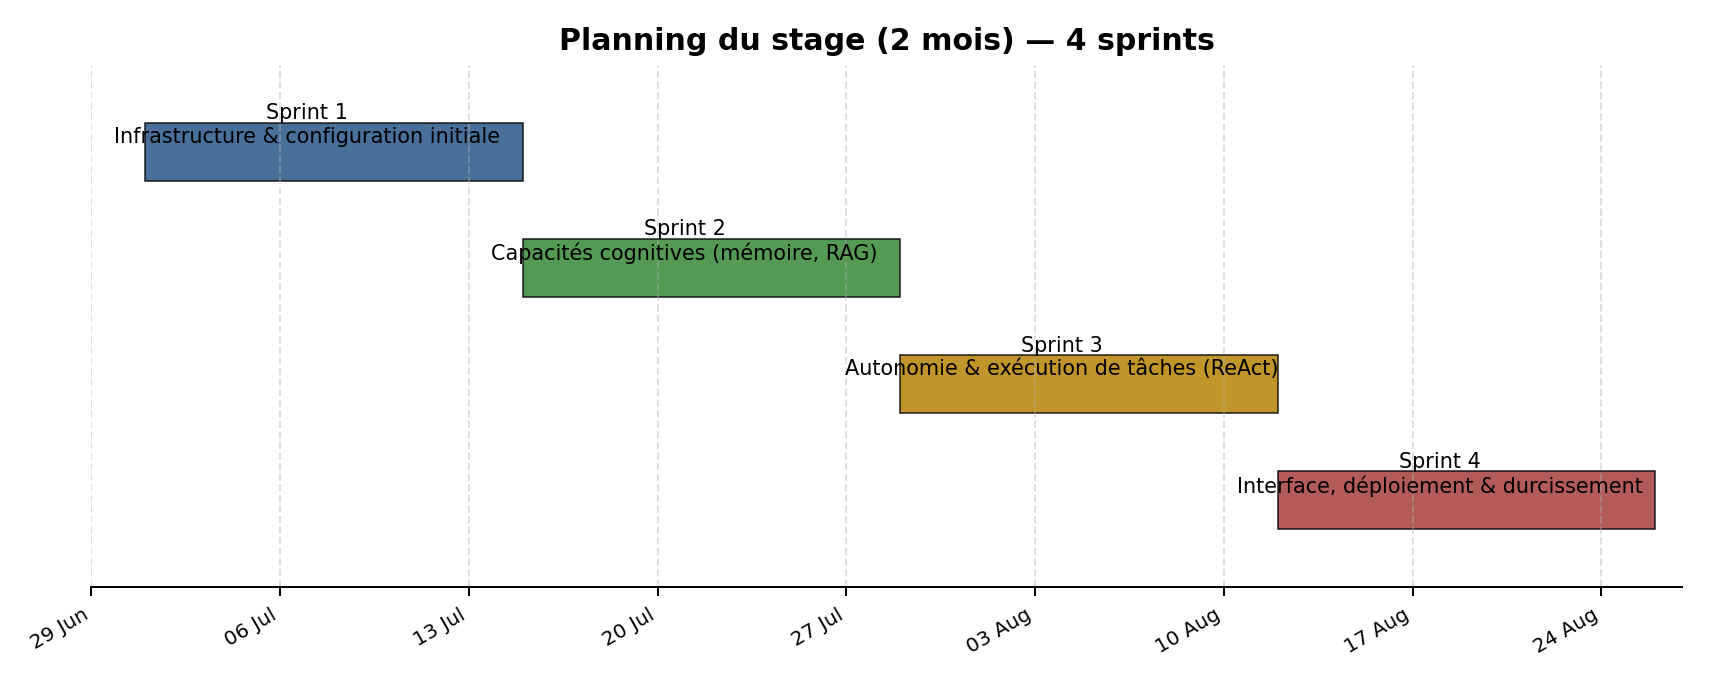
\includegraphics[width=0.95\linewidth]{diagrams/planning_sprints.png}
\caption{Planning prévisionnel du stage — 4 sprints de 2 semaines}
\label{fig:planning}
\end{figure}
\genfigure{Généré à partir des dates réelles du cahier des charges
(\texttt{diagrams/planning\_sprints.png}). Peut être remplacé par une
capture d'écran du tableau Jira / Confluence si l'entreprise en
dispose d'un plus détaillé.}

% =====================================================================
\chapter{Méthodologie de travail}
\label{chap:methodologie}
% =====================================================================

\section{Approche Agile et gestion de projet}

Le projet a été mené selon une approche \textbf{Agile / Scrum}
simplifiée, adaptée à un stage individuel : quatre sprints de deux
semaines, chacun aligné sur un \textit{Epic} du \textit{backlog}, avec
un point de synchronisation hebdomadaire avec le maître de stage.

\tocomplete{Décrire ici concrètement les rituels effectivement suivis
(point hebdomadaire, revue de sprint, rétrospective éventuelle) et les
outils de communication utilisés (Slack, Teams, email...).}

\section{Suivi via Jira}

Le \textit{backlog} a été structuré en 4 \textit{Epics}, eux-mêmes
décomposés en \textit{Stories} puis en \textit{Tasks} estimées en
jours. Le tableau \ref{tab:epics} synthétise cette hiérarchie.

\begin{table}[H]
\centering
\caption{Synthèse du backlog Jira par Epic}
\label{tab:epics}
\begin{tabularx}{\linewidth}{@{}l Y c c l@{}}
\toprule
\textbf{Clé} & \textbf{Epic} & \textbf{Stories} & \textbf{Tasks} & \textbf{Sprint} \\
\midrule
AGENT-EP-01 & Setup AWS \& Configuration Bedrock & 1 & 3 & Sprint 1 \\
AGENT-EP-02 & Développement de l'agent \& outils & 2 & 6 & Sprint 2--3 \\
AGENT-EP-03 & Mémoire \& persistance & 2 & 4 & Sprint 2 \\
AGENT-EP-04 & Déploiement serverless \& API & 1 & 3 & Sprint 4 \\
\bottomrule
\end{tabularx}
\end{table}

Le cahier des charges définit également quatre \textit{User Stories}
transverses (tableau \ref{tab:us}), rédigées au format
\textit{persona / action / bénéfice} avec critères d'acceptance en
notation \textit{Given/When/Then}.

\begin{table}[H]
\centering
\caption{User Stories principales et critères d'acceptance résumés}
\label{tab:us}
\begin{tabularx}{\linewidth}{@{}l Y Y@{}}
\toprule
\textbf{ID} & \textbf{User Story} & \textbf{Critère d'acceptance clé} \\
\midrule
US-01 & En tant qu'utilisateur, je veux poser une question
multi-étapes, afin que l'agent la décompose et mobilise les bons
outils. & $\geq 2$ outils différents exécutés, réponse en $< 30$\,s,
trace Thought/Action/Observation visible. \\
US-02 & En tant qu'utilisateur, je veux reprendre une conversation
interrompue, afin que l'agent se souvienne du contexte. & Accès aux 5
derniers échanges sans les renvoyer explicitement ; recherche en
mémoire long terme fonctionnelle. \\
US-03 & En tant que développeur, je veux ajouter un nouvel outil sans
refactoriser l'existant. & Outil conforme à l'interface \texttt{Tool}
utilisé automatiquement si pertinent ; appel journalisé dans
DynamoDB. \\
US-04 & En tant qu'opérateur, je veux consulter les logs en temps
réel, afin de détecter boucles et erreurs. & Étapes ReAct visibles
dans CloudWatch avec horodatage ; boucle détectée (même action
3$\times$) $\Rightarrow$ arrêt propre. \\
\bottomrule
\end{tabularx}
\end{table}

\tocomplete{Insérer ici une capture d'écran du tableau Jira (vue
Kanban ou Backlog) montrant les Epics/Stories/Tasks réellement
utilisés, ainsi qu'une capture de l'historique des commits Git montrant
la fréquence des livraisons.}

% =====================================================================
\chapter{Conception de la solution}
\label{chap:conception}
% =====================================================================

\section{Vue d'ensemble de l'architecture}

Le système repose sur une architecture \textbf{serverless} centrée
autour d'une fonction \textbf{AWS Lambda} packagée en image Docker,
exposée via une \textbf{Function URL} avec support du streaming de
réponse (nécessaire au protocole SSE). La figure \ref{fig:archi}
présente les composants principaux et leurs interactions.

\begin{figure}[H]
\centering
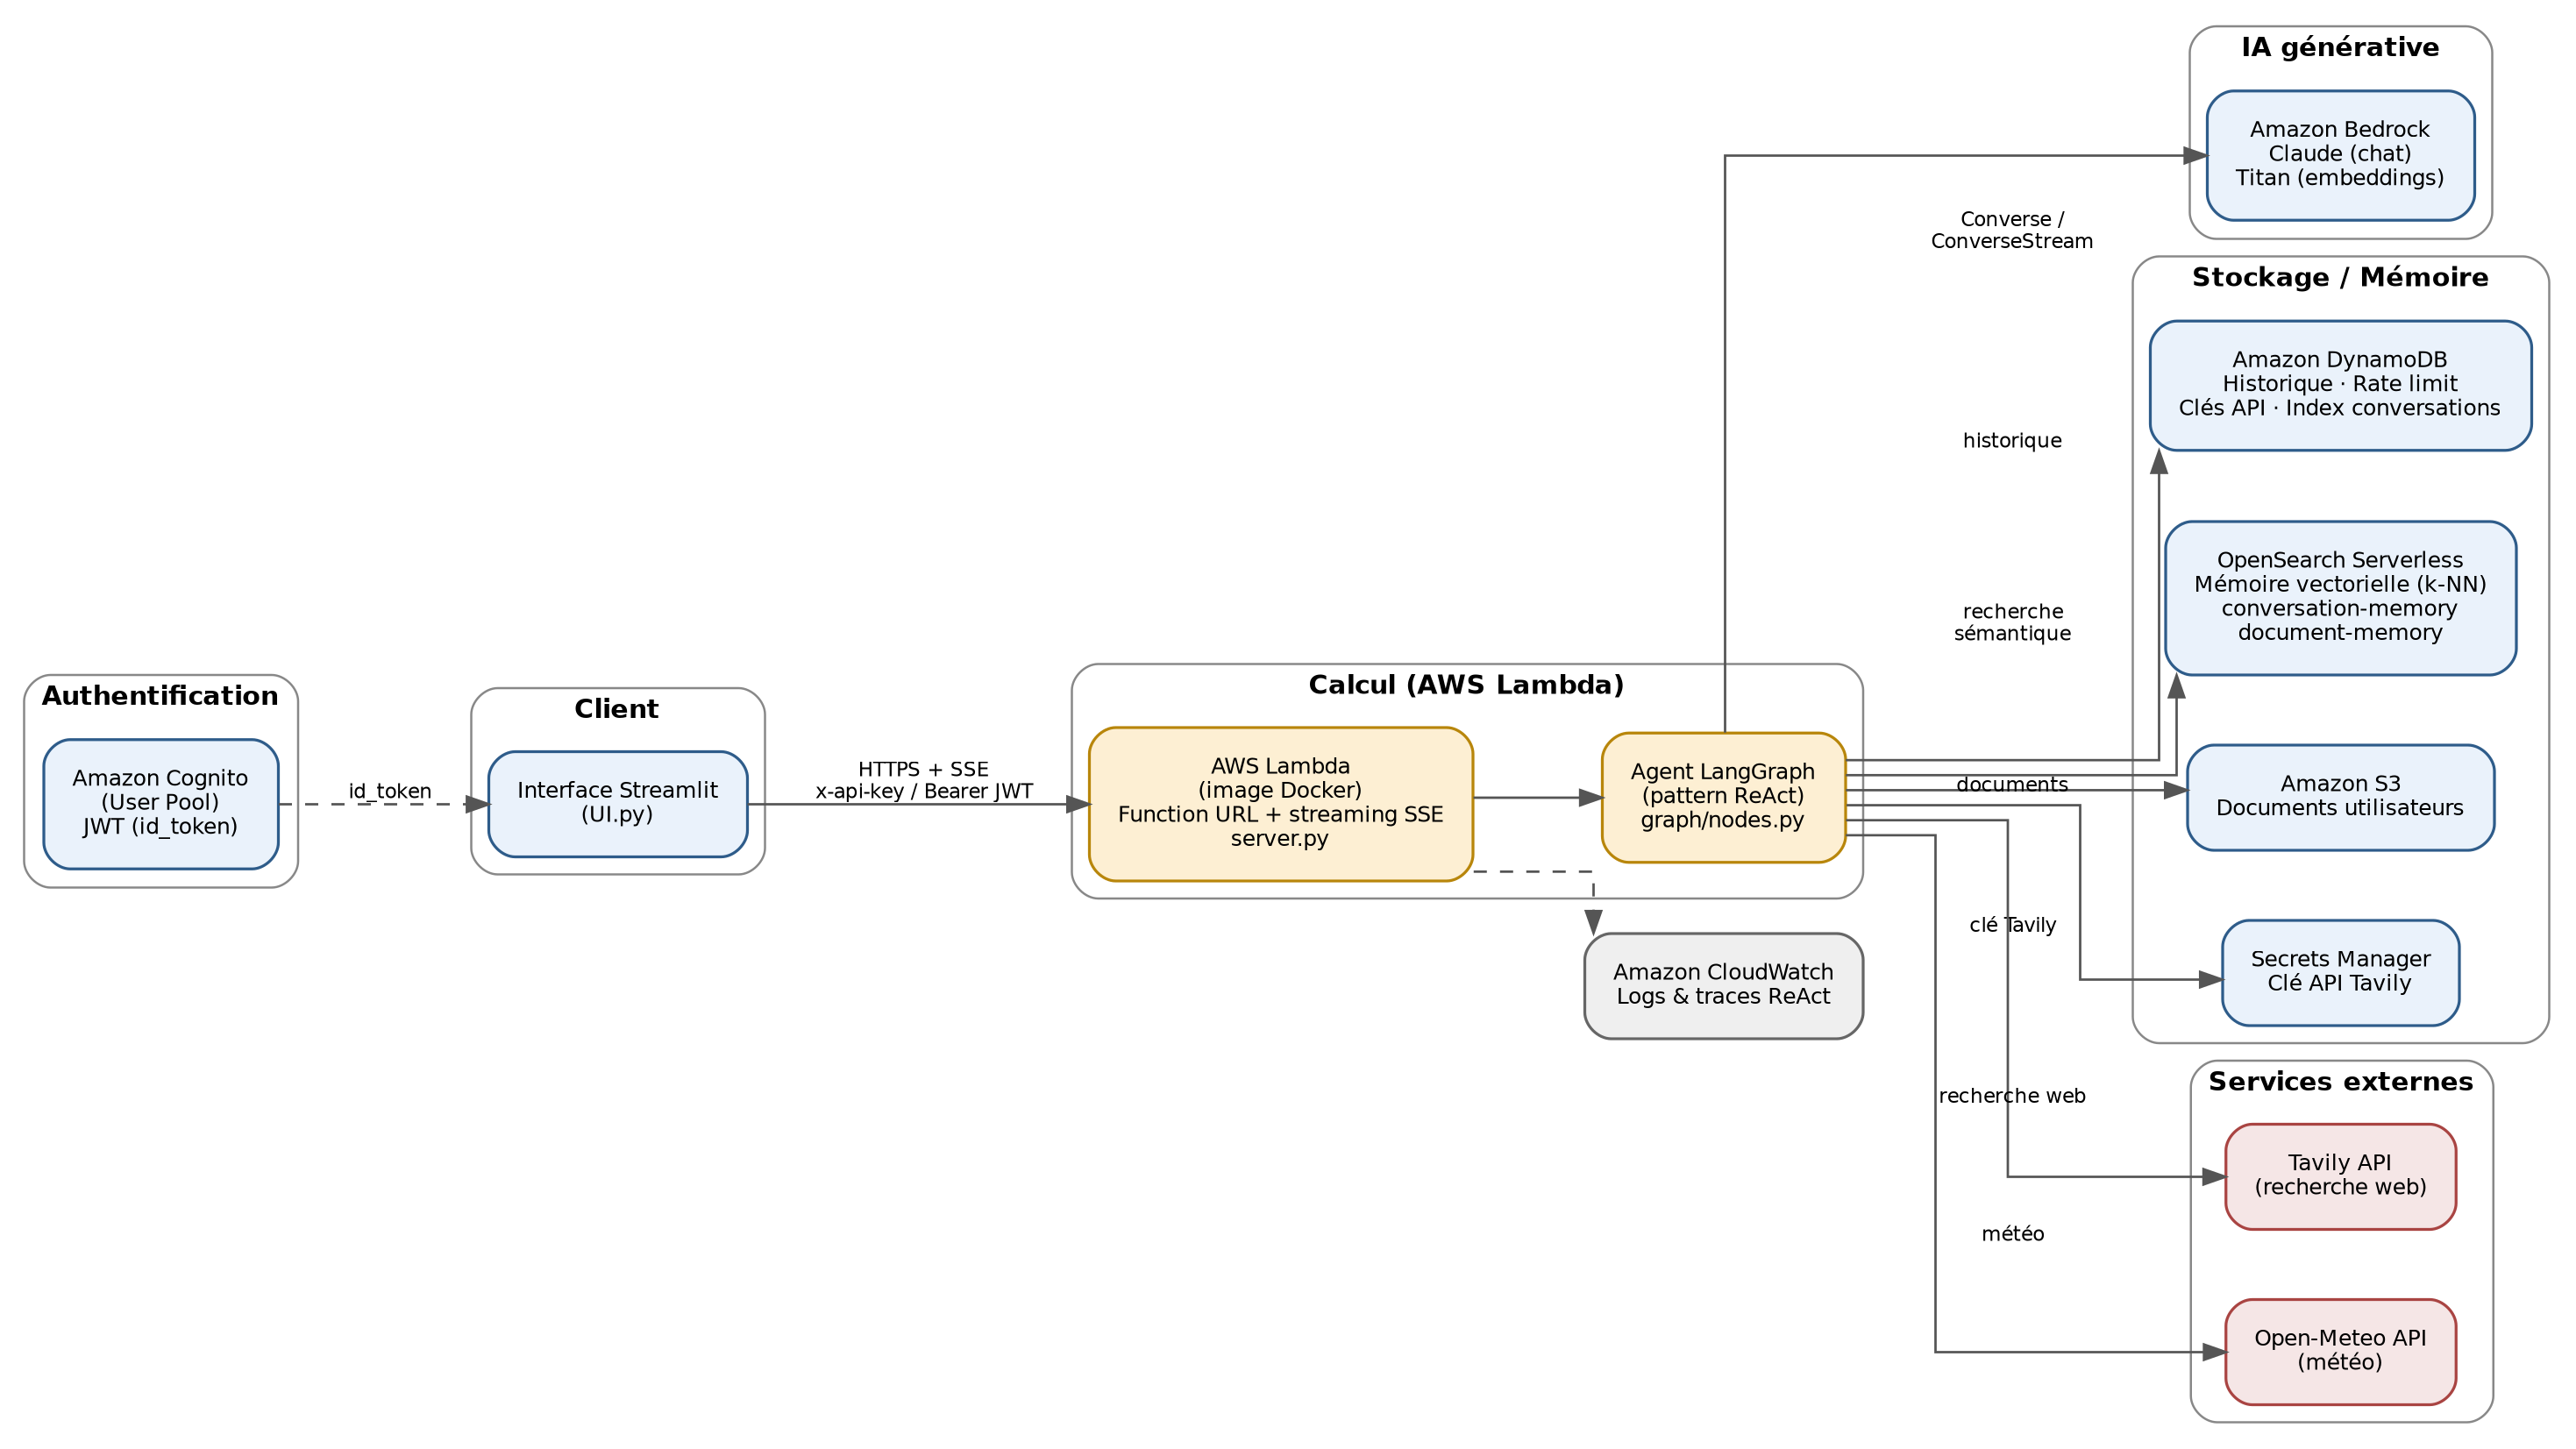
\includegraphics[width=\linewidth]{diagrams/architecture.png}
\caption{Architecture globale du système}
\label{fig:archi}
\end{figure}
\genfigure{Diagramme reconstitué à partir de l'analyse du code source
et de l'infrastructure CDK réellement déployée
(\texttt{diagrams/architecture.png}).}

\tocomplete{Si l'entreprise dispose d'un schéma d'architecture
officiel (dessiné sous draw.io / Lucidchart / AWS Architecture Icons
en amont du projet), l'ajouter ici en complément ou en remplacement,
et signaler explicitement les écarts éventuels entre le schéma prévu
et l'architecture réellement implémentée (cf. \S\ref{chap:ecarts}).}

\section{Composants principaux}

\begin{itemize}[nosep]
    \item \textbf{AWS Lambda (image Docker)} : héberge un serveur HTTP
    minimaliste (\texttt{server.py}, bibliothèque standard
    \texttt{http.server}) plutôt qu'un framework comme FastAPI, choix
    motivé par la nécessité de contrôler finement le streaming SSE des
    réponses.
    \item \textbf{Amazon Bedrock} : fournit l'accès managé au modèle
    de chat (Claude, via l'API \textit{Converse}/\textit{ConverseStream})
    et au modèle d'embedding (Titan) utilisé pour la mémoire
    sémantique.
    \item \textbf{Amazon DynamoDB} (4 tables) : historique brut des
    conversations, compteurs de limitation de débit, clés API valides,
    index des conversations par utilisateur.
    \item \textbf{Amazon OpenSearch Serverless} : mémoire vectorielle
    (recherche par similarité $k$-NN) pour la mémoire sémantique long
    terme et la base de connaissance interne.
    \item \textbf{Amazon S3} : stockage des documents uploadés par les
    utilisateurs.
    \item \textbf{Amazon Cognito} : authentification des utilisateurs
    (JWT), au-delà du périmètre initial du cahier des charges (cf.
    \S\ref{chap:ecarts}).
    \item \textbf{AWS Secrets Manager} : stockage sécurisé de la clé
    API Tavily (recherche web).
    \item \textbf{Amazon CloudWatch} : centralisation des logs et des
    traces structurées de la boucle ReAct.
    \item \textbf{Interface Streamlit} : application cliente de
    démonstration, consommant l'API en streaming.
\end{itemize}

\section{Modèle de données}

Le système combine un stockage relationnel-clé (DynamoDB, pour
l'historique brut et les métadonnées) et un stockage vectoriel
(OpenSearch Serverless, pour la recherche sémantique). La figure
\ref{fig:donnees} détaille le schéma logique de chaque table et index.

\begin{figure}[H]
\centering
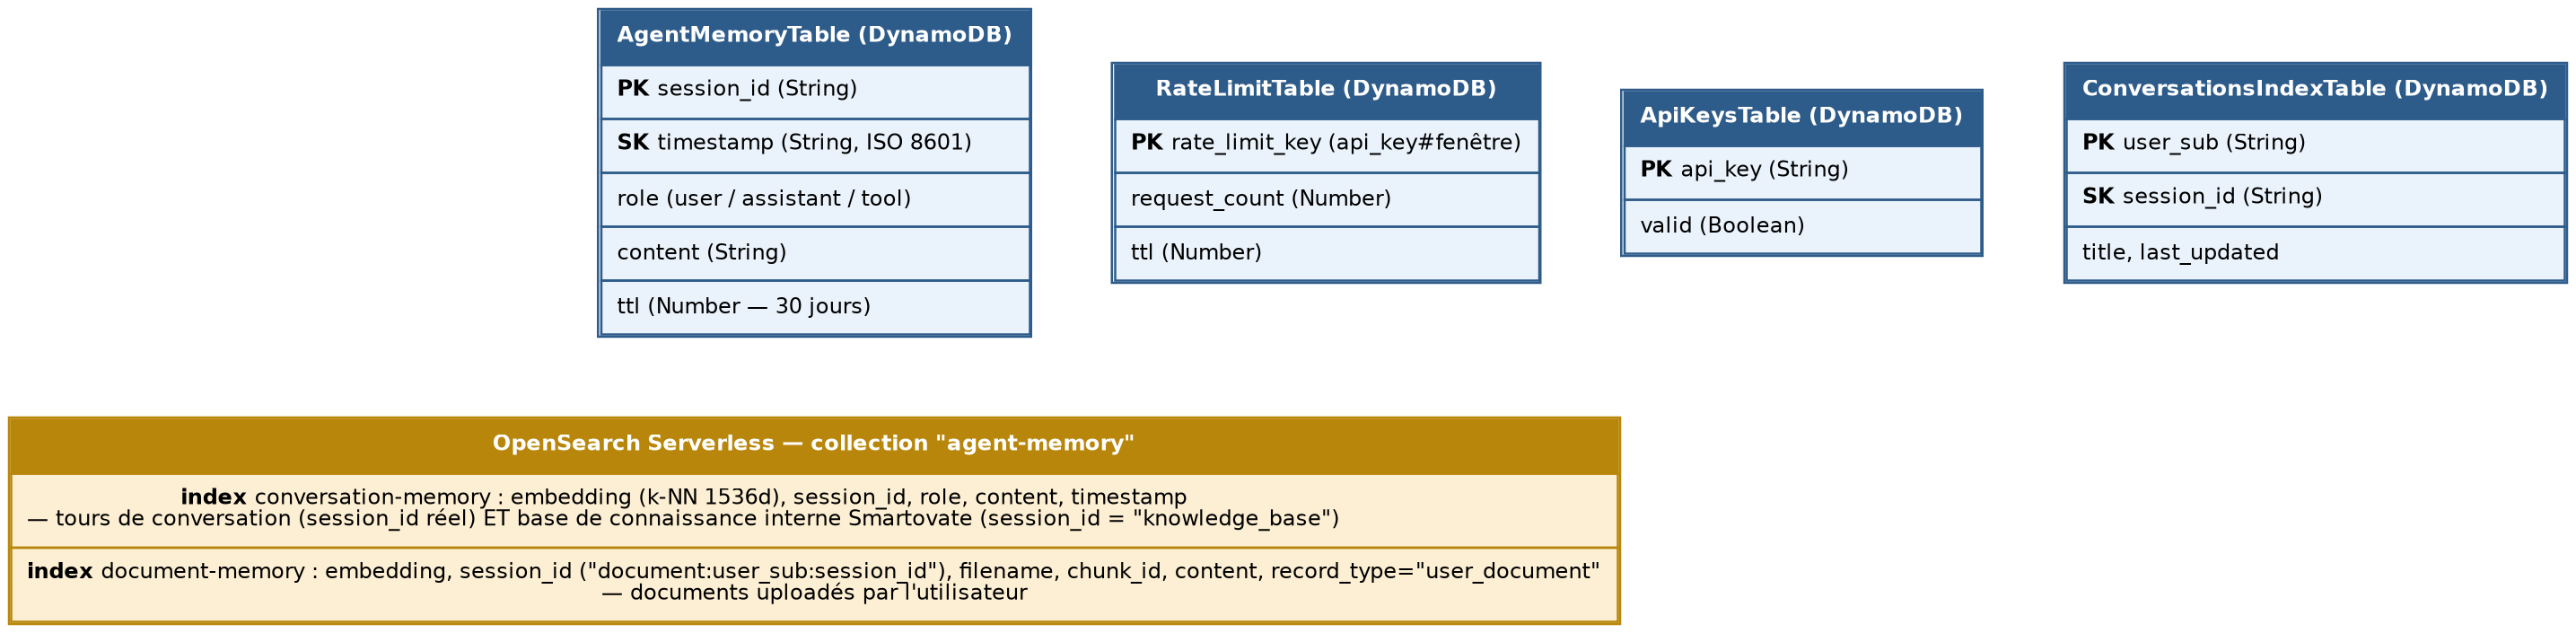
\includegraphics[width=\linewidth]{diagrams/modele_donnees.png}
\caption{Modèle de données — DynamoDB et OpenSearch Serverless}
\label{fig:donnees}
\end{figure}
\genfigure{Schéma extrait directement de l'implémentation
(\texttt{config.py}, \texttt{opensearch\_config.py}, \texttt{aws\_ai\_agent\_stack.py})
— \texttt{diagrams/modele\_donnees.png}.}

Un choix de conception notable concerne le \textbf{stockage des
embeddings} : ceux-ci ne sont jamais persistés dans DynamoDB (qui ne
propose pas de recherche vectorielle native), mais exclusivement dans
l'index OpenSearch dédié — décision qui a nécessité une correction en
cours de stage (\S\ref{sec:bug-embeddings}).

\section{Le patron ReAct et son orchestration par LangGraph}

L'agent est implémenté comme une machine à états \textbf{LangGraph},
alternant entre un nœud d'appel au modèle de langage
(\texttt{call\_model}) et un nœud d'exécution d'outil
(\texttt{call\_tools}), jusqu'à obtention d'une réponse finale. Deux
garde-fous protègent le système contre les comportements pathologiques
d'un agent autonome :

\begin{itemize}[nosep]
    \item un \textbf{plafond d'itérations} (10 par défaut, 20 au
    maximum), au-delà duquel l'agent s'arrête et explique la raison de
    l'arrêt à l'utilisateur ;
    \item une \textbf{détection de boucle} : si le même outil est
    appelé trois fois de suite avec des arguments strictement
    identiques, l'agent interrompt son exécution plutôt que de
    consommer indéfiniment des ressources (et du budget Bedrock).
\end{itemize}

\begin{figure}[H]
\centering
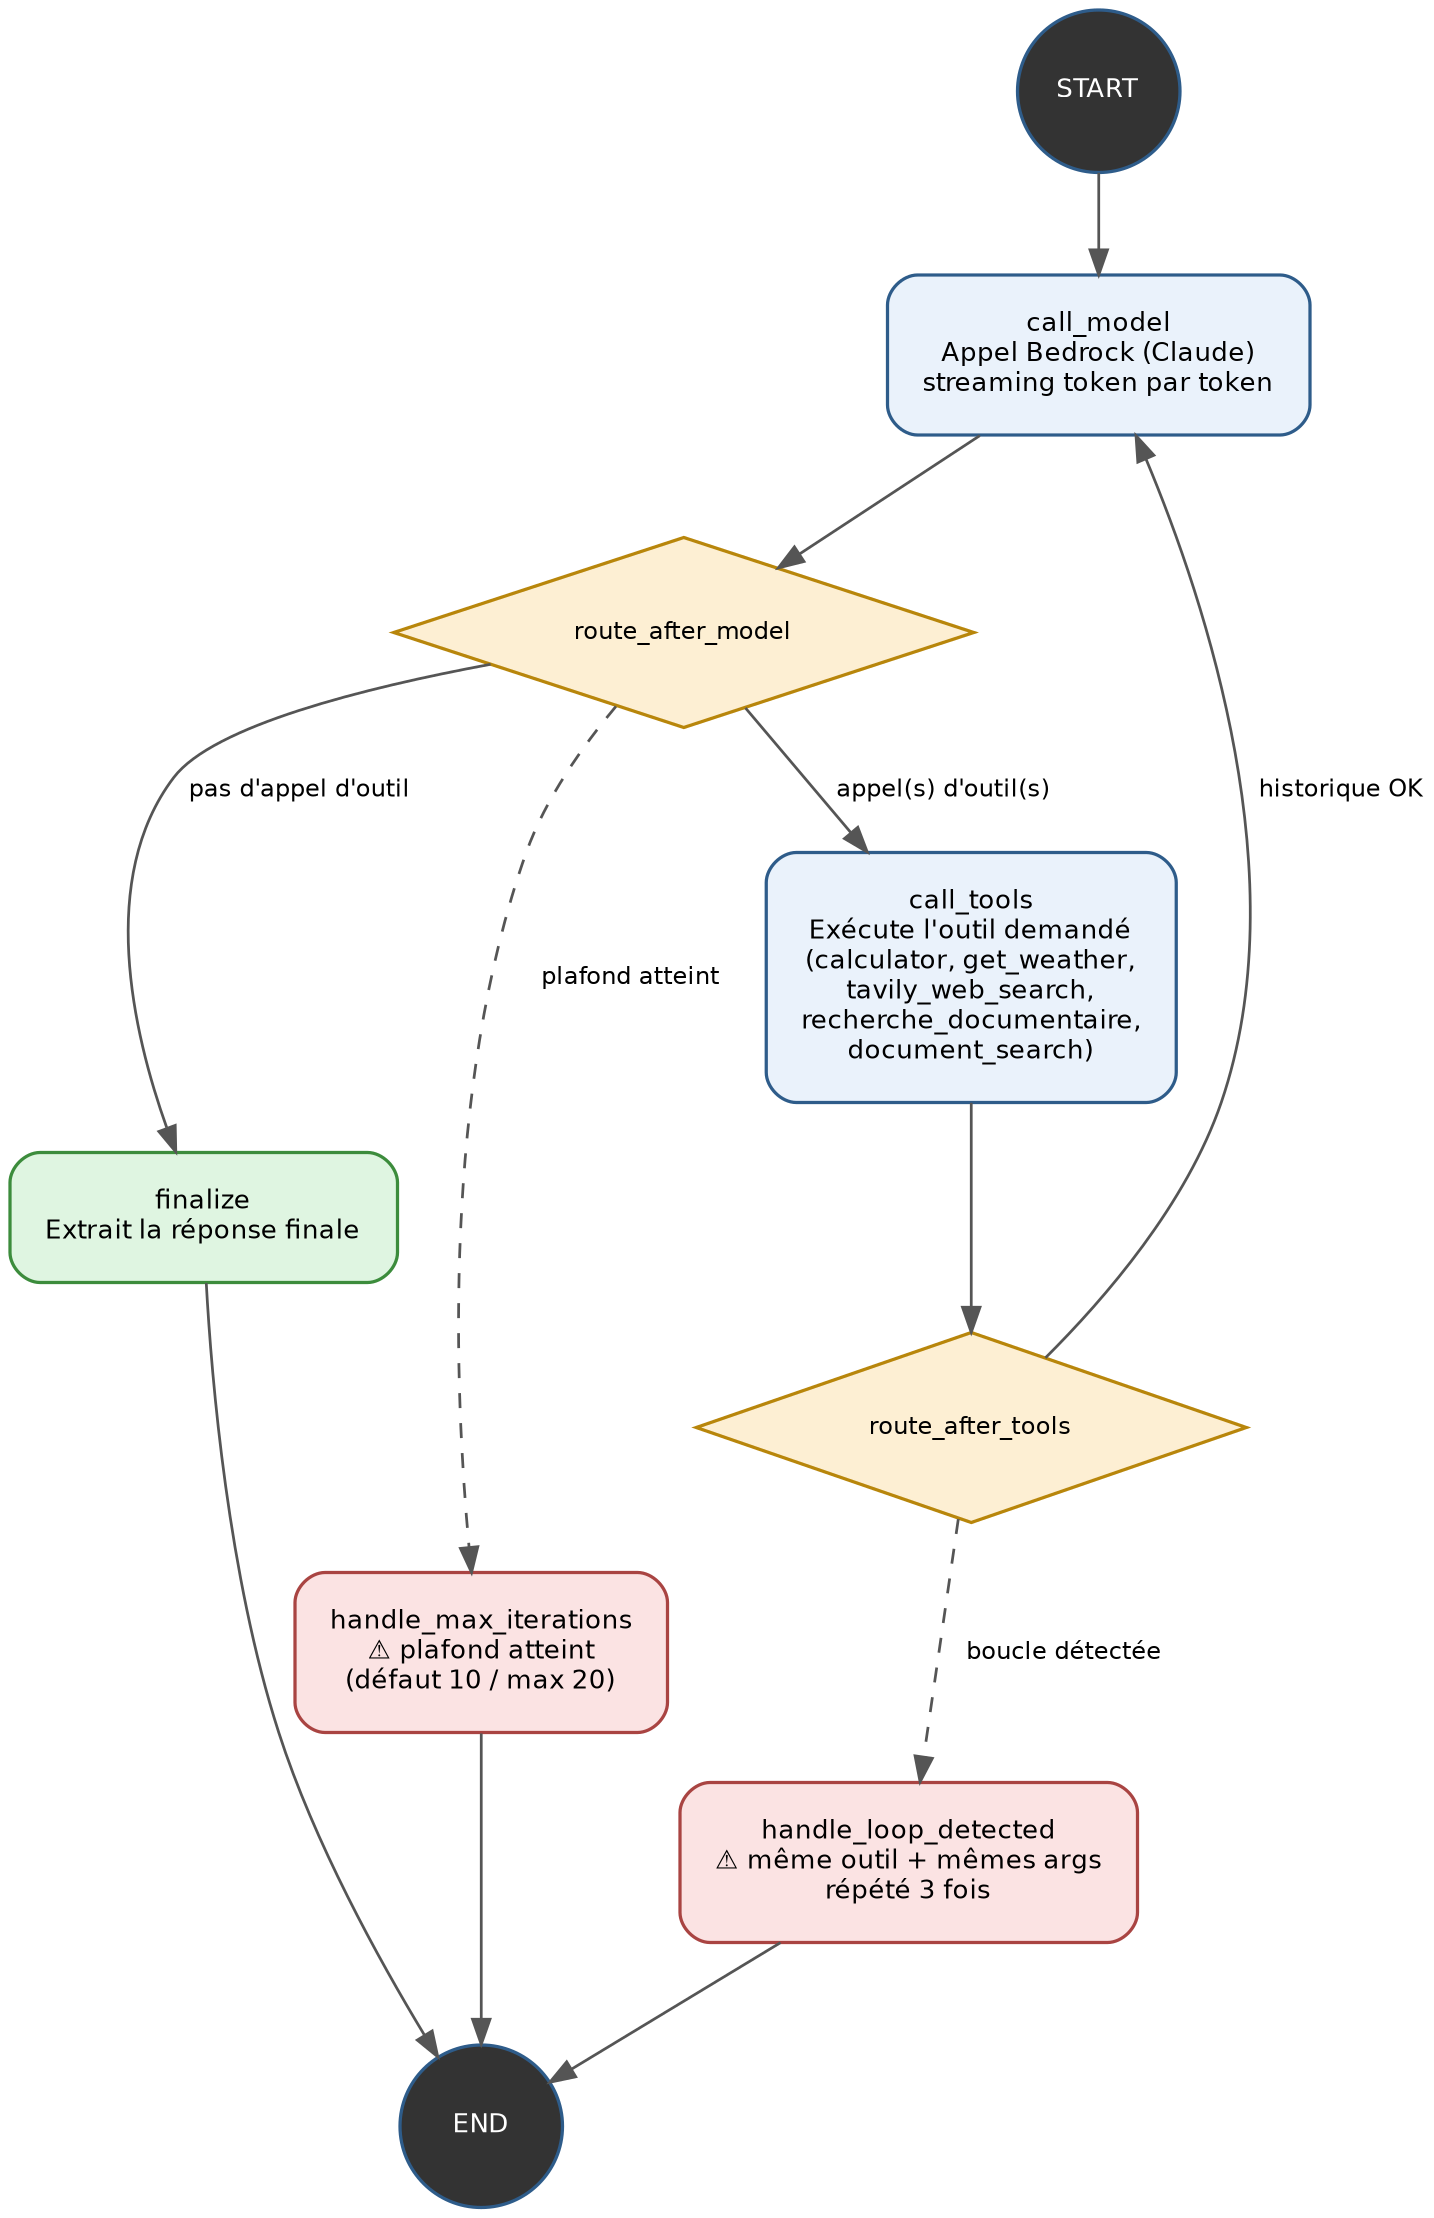
\includegraphics[width=0.85\linewidth]{diagrams/pipeline_react.png}
\caption{Pipeline ReAct implémenté avec LangGraph (\texttt{graph/nodes.py})}
\label{fig:pipeline}
\end{figure}
\genfigure{Diagramme d'état reconstitué à partir du code source
(\texttt{graph/nodes.py}, fonctions \texttt{route\_after\_model} et
\texttt{route\_after\_tools}) — \texttt{diagrams/pipeline\_react.png}.}

Le code~\ref{lst:loop} illustre la logique de détection de boucle,
volontairement simple (comparaison des trois derniers appels
d'outils, indépendante de l'ordre des clés grâce à
\texttt{json.dumps(..., sort\_keys=True)}).

\begin{lstlisting}[caption={Détection de boucle (\texttt{graph/nodes.py})}, label={lst:loop}]
LOOP_THRESHOLD = 3

def route_after_tools(state: AgentState) -> str:
    history = state["tool_call_history"]
    if len(history) < LOOP_THRESHOLD:
        return "call_model"
    last_n = history[-LOOP_THRESHOLD:]
    signatures = {
        json.dumps({"tool": c["tool"], "args": c["args"]}, sort_keys=True)
        for c in last_n
    }
    if len(signatures) == 1:
        return "loop_detected"
    return "call_model"
\end{lstlisting}

\section{Les cinq outils de l'agent}

\begin{table}[H]
\centering
\caption{Outils mis à disposition de l'agent}
\begin{tabularx}{\linewidth}{@{}l Y@{}}
\toprule
\textbf{Outil} & \textbf{Rôle} \\
\midrule
\texttt{calculator} & Évaluation d'expressions arithmétiques via
\texttt{ast}, avec une liste blanche stricte de nœuds autorisés (aucun
\texttt{eval()} brut). \\
\texttt{get\_weather} & Météo en temps réel (géocodage + prévisions)
via l'API Open-Meteo. \\
\texttt{tavily\_web\_search} & Recherche web via l'API Tavily, clé
récupérée depuis Secrets Manager. \\
\texttt{recherche\_documentaire} & RAG sur la base de connaissance
interne de Smartovate (index OpenSearch \texttt{conversation-memory},
espace de noms \texttt{knowledge\_base}). \\
\texttt{document\_search} & RAG sur les documents uploadés par
l'utilisateur (index OpenSearch \texttt{document-memory}), avec
stratégie de nouvelles tentatives pour absorber la latence
d'indexation \textit{quasi} temps réel d'OpenSearch. \\
\bottomrule
\end{tabularx}
\end{table}

\section{Sécurité}

Trois mécanismes protègent l'API : \textbf{authentification Cognito}
(JWT vérifié à chaque requête), \textbf{clé API} applicative, et
\textbf{limitation de débit} (100 requêtes/minute par clé, avec
stratégie \textit{fail-open} : une panne de DynamoDB ne bloque jamais
l'agent). Le principe du \textbf{moindre privilège} a été appliqué à
l'ensemble des permissions IAM de la fonction Lambda (\S\ref{chap:difficultes}).

% =====================================================================
\chapter{Réalisation}
\label{chap:realisation}
% =====================================================================

Ce chapitre détaille l'implémentation, organisée selon les quatre
\textit{Epics} du \textit{backlog} (tableau \ref{tab:epics}).

\section{Epic 1 — Setup AWS \& Configuration Bedrock}

Cette première étape a consisté à provisionner, sous forme de code
(\textbf{AWS CDK}, Python), l'ensemble de l'infrastructure : rôle IAM
de la fonction Lambda, activation de l'accès aux modèles Bedrock
(Claude, Titan), tables DynamoDB, collection OpenSearch Serverless
(avec ses trois politiques obligatoires : chiffrement, réseau, accès),
bucket S3, secret Tavily. L'ensemble du stack tient dans un unique
fichier \texttt{aws\_ai\_agent\_stack.py}, ce qui facilite sa relecture
mais a nécessité une vigilance particulière sur la portée des
permissions accordées (\S\ref{sec:bug-iam}).

\tocomplete{Capture d'écran de la console AWS Bedrock montrant les
modèles Claude/Titan activés, et capture du résultat de
\texttt{cdk deploy} en console.}

\section{Epic 2 — Développement de l'agent et de ses outils}

Le cœur de l'agent repose sur \textbf{LangGraph} plutôt que sur
l'\texttt{AgentExecutor} historique de LangChain mentionné dans le
cahier des charges — ce choix, plus moderne, permet un contrôle
explicite du graphe d'états (garde-fous, routage conditionnel) que ne
permet pas l'API haut niveau de LangChain. Chaque outil est exposé au
LLM via le décorateur \texttt{@tool} de \texttt{langchain\_core}
(équivalent fonctionnel à une classe héritant de \texttt{BaseTool},
avec une syntaxe plus concise). Le listing \ref{lst:calculator}
illustre le traitement défensif appliqué à l'outil le plus sensible en
matière de sécurité.

\begin{lstlisting}[caption={Extrait de la liste blanche de \texttt{calculator} (\texttt{tools/calculator.py})}, label={lst:calculator}]
_ALLOWED_NODES = (
    ast.Expression, ast.BinOp, ast.UnaryOp, ast.Constant,
    ast.Add, ast.Sub, ast.Mult, ast.Div, ast.Pow, ast.Mod,
    ast.USub, ast.UAdd,
)

def _safe_eval(expression: str) -> float:
    tree = ast.parse(expression, mode="eval")
    for node in ast.walk(tree):
        if not isinstance(node, _ALLOWED_NODES):
            raise ValueError(f"Expression non autorisee : {ast.dump(node)}")
    return eval(compile(tree, "<calculator>", "eval"))
\end{lstlisting}

\section{Epic 3 — Mémoire et persistance}

La mémoire court terme (fenêtre glissante des cinq derniers échanges,
conforme à la spécification F3 du cahier des charges) est implémentée
par une classe \texttt{DynamoDBChatMessageHistory} maison, plutôt que
par la classe \texttt{ConversationBufferWindowMemory} de LangChain
explicitement mentionnée dans le cahier des charges — celle-ci étant
désormais dépréciée par l'éditeur au profit du protocole
\texttt{BaseChatMessageHistory}, choix documenté dans le
\texttt{README.md} du projet.

La mémoire long terme s'appuie sur une recherche de similarité (
\textit{top-k}=3) dans l'index vectoriel OpenSearch, déclenchée avant
chaque réponse de l'agent pour retrouver le contexte le plus pertinent
parmi les échanges passés.

\tocomplete{Capture d'écran de la console DynamoDB (tables créées,
exemple d'item) et de la console OpenSearch Serverless (collection
\texttt{agent-memory}, indices créés).}

\section{Epic 4 — Déploiement serverless et API}

L'agent est empaqueté en image Docker et déployé sur AWS Lambda,
exposé via une \textbf{Function URL} avec mode d'invocation
\texttt{RESPONSE\_STREAM}, permettant l'envoi de la réponse au fil de
sa génération par le modèle (protocole SSE). L'interface Streamlit
consomme ce flux pour afficher la réponse token par token, avec un
indicateur de chargement pendant la phase de raisonnement.

\tocomplete{Capture d'écran de l'interface Streamlit en fonctionnement
(conversation en cours, réponse en cours de streaming), et capture de
la console Lambda montrant la fonction déployée et sa Function URL.}

% =====================================================================
\chapter{Tests et validation}
\label{chap:tests}
% =====================================================================

La stratégie de validation du système repose sur deux niveaux
complémentaires et volontairement distincts : des \textbf{tests
unitaires}, qui vérifient la logique du code indépendamment de tout
service externe réel, et un \textbf{harnais d'évaluation de bout en
bout}, qui interroge le système réellement déployé.

\section{Tests unitaires}

161 tests ont été écrits avec \texttt{pytest}, répartis en 11 fichiers
et couvrant l'ensemble des composants critiques (tableau
\ref{tab:tests}). Aucun appel réseau ou AWS réel n'est effectué : les
dépendances externes (Bedrock, OpenSearch, DynamoDB, Secrets Manager,
Open-Meteo, Tavily) sont systématiquement simulées
(\texttt{unittest.mock}), ce qui garantit une exécution rapide (moins
de 20 secondes pour la suite complète) et déterministe.

\begin{table}[H]
\centering
\caption{Répartition des tests unitaires par module}
\label{tab:tests}
\begin{tabularx}{\linewidth}{@{}l c c@{}}
\toprule
\textbf{Fichier de test} & \textbf{Nb tests} & \textbf{Couverture du module} \\
\midrule
\texttt{test\_calculator.py} & 20 & 100\,\% \\
\texttt{test\_weather.py} & 9 & 100\,\% \\
\texttt{test\_tavily\_web\_search.py} & 12 & 98\,\% \\
\texttt{test\_search.py} (RAG interne) & 8 & 100\,\% \\
\texttt{test\_document\_search.py} & 14 & 86\,\% \\
\texttt{test\_graph\_nodes.py} (cœur ReAct) & 23 & 85\,\% \\
\texttt{test\_memory\_service.py} & 16 & 87\,\% \\
\texttt{test\_rate\_limit\_service.py} & 11 & 100\,\% \\
\texttt{test\_utils.py} & 12 & 100\,\% \\
\texttt{test\_server\_stream.py} & 9 & --- \\
\texttt{test\_evaluation\_harness.py} & 27 & 100\,\% \\
\midrule
\textbf{Total} & \textbf{161} & \textbf{71\,\% (ensemble du dossier \texttt{lambda/})} \\
\bottomrule
\end{tabularx}
\end{table}

La couverture globale (71\,\%) reste en-deçà de l'objectif de 80\,\%
fixé par le cahier des charges ; l'écart est concentré sur les modules
d'authentification et le point d'entrée HTTP complet
(\texttt{server.py}), plus coûteux à tester unitairement du fait de
leurs nombreuses dépendances externes imbriquées (cf.
\S\ref{chap:ecarts}).

\tocomplete{Capture d'écran de l'exécution de \texttt{pytest -{}-cov}
en local montrant le résumé de couverture ligne par ligne.}

\section{Harnais d'évaluation de bout en bout}

Un second niveau de validation, spécifiquement demandé par le cahier
des charges (livrable «  Rapport d'évaluation  »), interroge le
système \textbf{réellement déployé} sur 23 scénarios représentatifs :
culture générale (aucun outil attendu), calculatrice, météo, recherche
web, RAG interne, enchaînement de plusieurs outils, mémoire
conversationnelle sur deux tours liés, respect du périmètre du
\textit{system prompt}, et robustesse (entrée invalide, tentative
d'injection). Chaque scénario dispose d'un critère de succès
automatisable (mots-clés attendus, outil déclenché ou non, rejet HTTP
propre).

\begin{figure}[H]
\centering
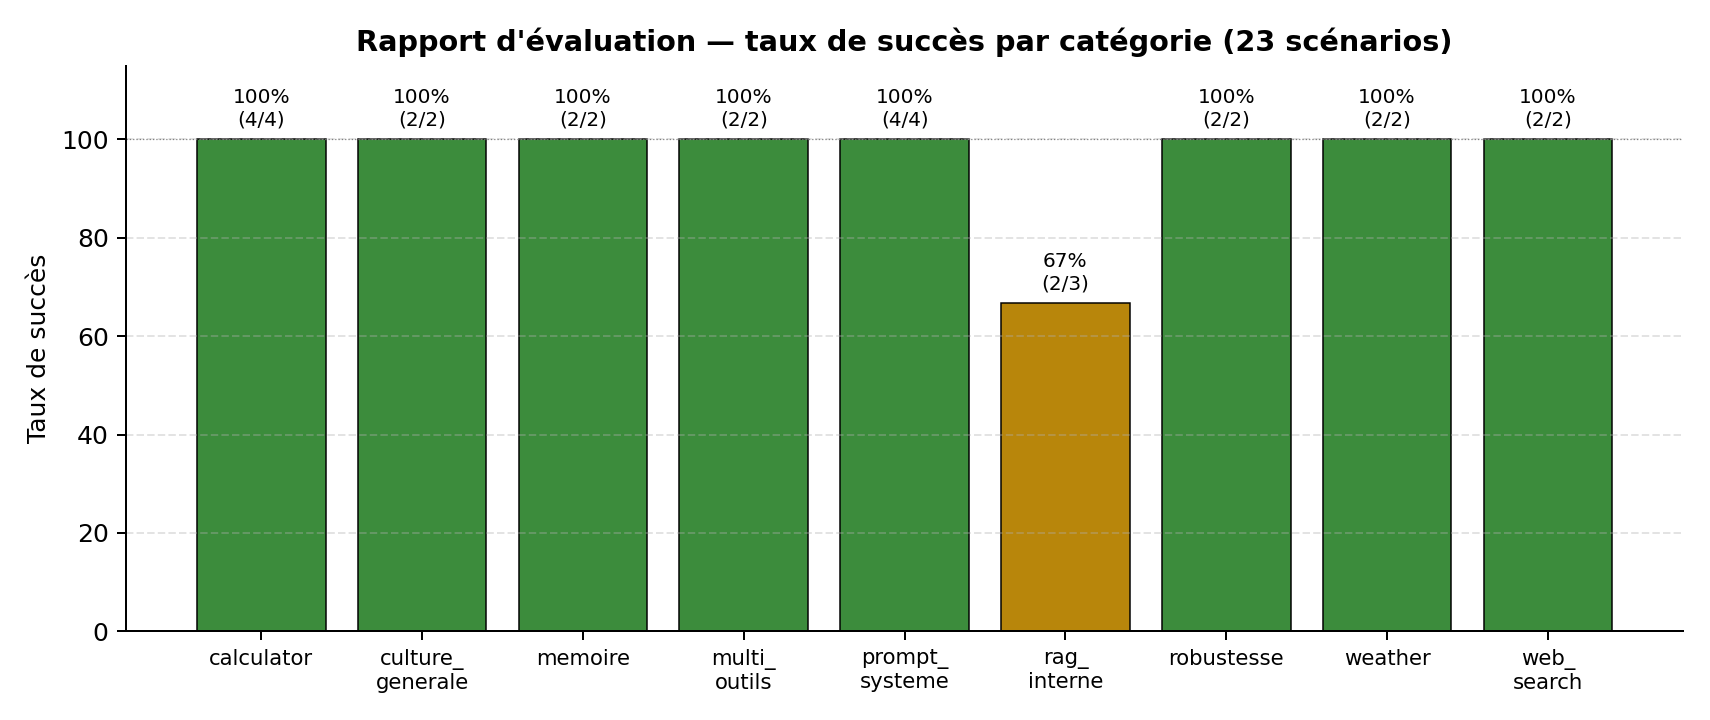
\includegraphics[width=\linewidth]{diagrams/resultats_evaluation.png}
\caption{Taux de succès par catégorie — dernière exécution (23 scénarios)}
\label{fig:eval}
\end{figure}
\genfigure{Généré à partir du fichier \texttt{rapport\_evaluation.csv}
produit par le harnais (\texttt{diagrams/resultats\_evaluation.png}).
À régénérer avec les données de la dernière exécution avant remise
finale du rapport.}

Le taux de succès global atteint \textbf{95,7\,\%} (22/23), pour une
latence moyenne de 8,1 secondes par requête (médiane 8,3 s, P95 à
11,7 s) — un temps de réponse cohérent avec un usage interactif,
d'autant que le temps avant le premier caractère affiché
(\textit{Time To First Token}) reste proche de 2,9 secondes en
médiane, ce qui donne à l'utilisateur une sensation de réactivité
correcte malgré une réponse complète plus longue à produire.

Le seul scénario en échec (\texttt{rag-02}, catégorie «  RAG interne
 ») est \textbf{informatif plutôt que révélateur d'un bug} : l'agent
interroge correctement sa base de connaissance, mais celle-ci ne
contient pas l'information demandée (les modèles de fondation utilisés
par Smartovate) ; l'agent répond alors honnêtement qu'il ne sait pas,
plutôt que d'halluciner une réponse — comportement souhaitable du
point de vue de la fiabilité, même s'il compte comme un échec au sens
strict du critère de test.

% =====================================================================
\chapter{Difficultés rencontrées et solutions}
\label{chap:difficultes}
% =====================================================================

Cette section documente les principales anomalies identifiées et
corrigées en cours de stage. Chacune a été découverte par une
combinaison de lecture de code, de tests ciblés et, pour certaines,
d'exécution réelle via le harnais d'évaluation — une démarche
méthodique qui constitue en elle-même un apprentissage important de ce
stage.

\section{Reconnexion silencieuse défaillante}

\textbf{Symptôme :} après un rafraîchissement de la page Streamlit,
l'utilisateur était systématiquement renvoyé à l'écran de connexion,
malgré la présence d'un jeton de rafraîchissement valide en cookie.

\textbf{Cause :} la bibliothèque de gestion de cookies utilisée
renvoie un dictionnaire vide (\texttt{\{\}}) par défaut tant que le
composant JavaScript sous-jacent n'a pas eu le temps de répondre — et
non \texttt{None}, comme le supposait le code de vérification
(\texttt{if cookies is None: st.stop()}). Ce test ne se déclenchait
donc jamais, et le code concluait à tort à l'absence de cookie dès le
premier cycle de rendu.

\textbf{Correction :} appel direct au composant sous-jacent avec un
\texttt{default=None} explicite, restaurant la logique d'attente
initialement prévue.

\section{Mémoire sémantique jamais indexée}
\label{sec:bug-embeddings}

\textbf{Symptôme :} la recherche sémantique sur l'historique des
conversations ne retournait jamais de résultat pertinent.

\textbf{Cause :} les \textit{embeddings} étaient bien calculés à
chaque tour de conversation, mais uniquement transmis à la fonction de
sauvegarde DynamoDB — jamais à \texttt{vector\_store.save\_document()},
la fonction responsable de l'indexation réelle dans OpenSearch. Le
chemin de production (\texttt{server.py}) désactivait même
explicitement ce paramètre (\texttt{user\_embedding=None}).

\textbf{Correction :} DynamoDB ne conserve désormais que le texte brut
(il n'offre pas de recherche vectorielle native), et un appel explicite
à \texttt{vector\_store.save\_document()} a été ajouté après chaque
tour de conversation, pour les messages utilisateur et assistant.

\section{Permissions IAM excessivement larges}
\label{sec:bug-iam}

\textbf{Symptôme :} la politique IAM de la fonction Lambda accordait
un accès complet (\texttt{dynamodb:*}, actions Bedrock, actions
OpenSearch) sur \textbf{toutes} les ressources du compte
(\texttt{Resource: "*"}), avec un commentaire du code indiquant
explicitement « à restreindre en production » — en contradiction
directe avec le critère d'acceptance de la toute première tâche du
projet («  les rôles et politiques IAM sont créés avec le principe de
moindre privilège  »).

\textbf{Correction :} chaque table DynamoDB dispose désormais d'une
permission scopée à son seul ARN (via les méthodes
\texttt{grant\_read\_write\_data} du CDK) ; la permission OpenSearch
(\texttt{aoss:APIAccessAll}, seule action IAM que propose AWS pour ce
service) est restreinte à l'ARN de l'unique collection utilisée ; les
permissions Bedrock sont limitées aux familles de modèles réellement
invoquées. Validation effectuée par synthèse du \textit{template}
CloudFormation généré et inspection automatisée de l'absence de tout
\texttt{Resource: "*"}.

\section{Secret d'API en clair dans le terminal}

\textbf{Symptôme :} la clé de l'API Tavily devait être ressaisie dans
le terminal (\texttt{\$env:TAVILY\_API\_KEY=...}) avant chaque
déploiement CDK.

\textbf{Correction :} la clé est désormais stockée une seule fois dans
\textbf{AWS Secrets Manager} ; le \textit{stack} CDK référence le
secret par son nom (jamais sa valeur), et la fonction Lambda le
récupère elle-même au démarrage, avec mise en cache mémoire pour la
durée de vie du conteneur d'exécution.

\section{Garde-fous de sécurité invisibles côté utilisateur}

\textbf{Symptôme :} lorsque l'un des deux garde-fous de la boucle
ReAct se déclenchait (plafond d'itérations atteint, ou boucle
détectée), l'utilisateur ne recevait \textbf{aucun message} — la bulle
de réponse restait vide dans l'interface, sans aucune explication.

\textbf{Cause :} le message d'explication généré par ces deux nœuds
terminaux n'est jamais produit par le modèle de langage (il s'agit
d'une chaîne de caractères Python fixe) et n'est donc jamais diffusé
via les événements de \textit{streaming} token par token qui
alimentent normalement l'affichage côté client ; le mécanisme de
récupération prévu dans le code testait par erreur le nom du mauvais
nœud du graphe.

\textbf{Correction :} émission explicite d'un évènement de type
«  token » contenant le message du garde-fou dès qu'un de ces deux
nœuds terminaux produit une réponse, sans dupliquer l'affichage sur le
chemin de succès normal.

\section{Encodage des caractères corrompu}

\textbf{Symptôme :} les caractères accentués et les émojis
apparaissaient corrompus dans les réponses de l'agent (par exemple
«  é » affiché «  é »), constaté concrètement dans les
réponses collectées par le harnais d'évaluation.

\textbf{Cause :} l'en-tête HTTP \texttt{Content-Type} du flux SSE
n'annonçait pas explicitement l'encodage UTF-8 utilisé pour encoder le
corps de la réponse ; un client HTTP sans indication d'encodage
retombe par défaut sur Latin-1, provoquant une réinterprétation
erronée, octet par octet, de tout caractère non-ASCII.

\textbf{Correction :} ajout explicite de \texttt{charset=utf-8} à
l'en-tête \texttt{Content-Type} des réponses HTTP et du flux SSE.

\section{Synthèse}

\begin{table}[H]
\centering
\caption{Synthèse des anomalies corrigées durant le stage}
\begin{tabularx}{\linewidth}{@{}l Y c@{}}
\toprule
\textbf{Anomalie} & \textbf{Impact} & \textbf{Sévérité} \\
\midrule
Reconnexion silencieuse cassée & Ré-authentification systématique & Élevée \\
Embeddings jamais indexés & Mémoire sémantique inopérante & Élevée \\
IAM \texttt{Resource: "*"} & Surface d'attaque excessive & Élevée \\
Secret Tavily en clair & Friction opérationnelle, risque de fuite & Moyenne \\
Garde-fous invisibles & Réponse vide sans explication & Élevée \\
Encodage UTF-8 cassé & Caractères corrompus & Moyenne \\
\bottomrule
\end{tabularx}
\end{table}

Chacune de ces corrections est verrouillée par au moins un test de
non-régression, garantissant qu'elle ne pourra être réintroduite sans
faire échouer immédiatement la suite de tests.

% =====================================================================
\chapter{Écarts par rapport au cahier des charges}
\label{chap:ecarts}
% =====================================================================

Par souci de transparence, ce chapitre recense les écarts assumés ou
constatés entre les spécifications du cahier des charges et le système
effectivement livré.

\section{AWS API Gateway défini mais non utilisé en production}
\label{sec:ecart-apigw}

Le cahier des charges prescrit explicitement AWS API Gateway comme
point d'entrée HTTP. Une ressource \texttt{RestApi} est bien définie
dans le \textit{stack} CDK (clé API, plan d'utilisation, limitation de
débit), mais l'interface Streamlit interroge en réalité directement la
\textbf{Function URL} de la fonction Lambda. Ce choix découle d'une
contrainte technique réelle : le streaming de réponse token par token
(SSE) n'est pas nativement supporté par l'API Gateway REST classique,
alors qu'il l'est par les Function URLs Lambda en mode
\texttt{RESPONSE\_STREAM}. La ressource API Gateway laissée dans le
\textit{stack} constitue toutefois une zone d'ombre à clarifier
(suppression ou finalisation) avant toute mise en production ultérieure.

\section{TTL de la mémoire conversationnelle}

Le cahier des charges spécifie un TTL de 7 jours pour la mémoire
utilisateur en DynamoDB ; l'implémentation actuelle utilise 30 jours.

\section{Couverture de tests}

L'objectif de 80\,\% de couverture n'est atteint que sur les modules
critiques (outils, cœur ReAct, mémoire, limitation de débit — 85 à
100\,\%) ; la couverture globale du dossier \texttt{lambda/} est de
71\,\%, les modules d'authentification et le point d'entrée HTTP
complet restant partiellement non couverts.

\section{Documentation API}

Le cahier des charges et le \textit{backlog} Jira mentionnent une
documentation Swagger/OpenAPI de l'API. Le passage à un serveur HTTP
natif Python (plutôt que FastAPI, pour les raisons de streaming
évoquées en \S\ref{sec:ecart-apigw}) a fait perdre la génération
automatique de cette documentation ; aucune spécification OpenAPI
écrite à la main ne la remplace à ce jour.

\section{Extensions au-delà du périmètre initial}

À l'inverse, certains éléments livrés dépassent le périmètre du cahier
des charges : authentification multi-utilisateur via Amazon Cognito
(non demandée explicitement), isolement strict des documents et
conversations par utilisateur, et harnais d'évaluation automatisé
réutilisable (au-delà d'un simple rapport ponctuel).

% =====================================================================
\chapter{Bilan et compétences acquises}
% =====================================================================

\section{Compétences techniques}

\begin{itemize}[nosep]
    \item Conception et exploitation d'un agent conversationnel basé
    sur le patron ReAct, avec LangChain / LangGraph ;
    \item utilisation opérationnelle d'AWS Bedrock (modèles de chat et
    d'embedding, API \textit{Converse}) ;
    \item infrastructure-as-code avec AWS CDK (Python), incluant la
    configuration d'OpenSearch Serverless et la gestion fine des
    permissions IAM ;
    \item conception d'une architecture serverless avec streaming HTTP
    (Server-Sent Events) ;
    \item méthodologie de test logicielle : tests unitaires avec
    simulation systématique des dépendances externes, conception d'un
    harnais d'évaluation de bout en bout avec métriques objectives ;
    \item diagnostic et correction d'anomalies dans un système
    distribué (authentification, streaming, encodage, sécurité IAM).
\end{itemize}

\section{Compétences transversales}

\tocomplete{Compléter avec les compétences propres au vécu du stage :
gestion du temps sur 8 semaines, communication avec le maître de
stage, autonomie dans la priorisation des tâches, etc.}

% =====================================================================
\chapter{Conclusion et perspectives}
% =====================================================================

Ce stage de deux mois a permis de livrer un agent IA autonome
fonctionnel, répondant à l'essentiel des exigences du cahier des
charges initial : architecture ReAct avec garde-fous, mémoire hybride
court/long terme, cinq outils opérationnels, interface de
démonstration en streaming, et déploiement effectif sur
l'infrastructure AWS de Smartovate Ltd. Au-delà du strict périmètre
fonctionnel, une part substantielle du travail a consisté à fiabiliser
un système déjà partiellement construit : 161 tests unitaires, un
harnais d'évaluation à 23 scénarios (95,7\,\% de réussite en
conditions réelles), et la correction de six anomalies fonctionnelles
et de sécurité significatives.

Les principales pistes d'amélioration identifiées à l'issue du stage
sont : porter la couverture de tests à 80\,\% sur l'ensemble du code
(notamment le serveur HTTP et l'authentification), clarifier le
positionnement d'API Gateway dans l'architecture, documenter l'API au
format OpenAPI, et mettre en place les mécanismes de maîtrise des
coûts recommandés par le registre de risques du cahier des charges
(budgets AWS, \textit{Provisioned Concurrency}).

\tocomplete{Conclure par une réflexion personnelle sur l'apport du
stage au projet professionnel, et les suites envisagées (poursuite
avec Smartovate, autres opportunités, etc.).}

% ===================== BIBLIOGRAPHIE =====================
\begin{thebibliography}{9}

\bibitem{yao2022react}
Yao, S., Zhao, J., Yu, D., Du, N., Shafran, I., Narasimhan, K., \& Cao, Y.
\textit{ReAct: Synergizing Reasoning and Acting in Language Models}.
arXiv:2210.03629, 2022.

\bibitem{langchain}
LangChain / LangGraph — Documentation officielle.
\url{https://python.langchain.com} et \url{https://langchain-ai.github.io/langgraph/}

\bibitem{bedrock}
AWS. \textit{Amazon Bedrock — User Guide}.
\url{https://docs.aws.amazon.com/bedrock/}

\bibitem{opensearch}
AWS. \textit{Amazon OpenSearch Serverless — Developer Guide}.
\url{https://docs.aws.amazon.com/opensearch-service/}

\bibitem{cdk}
AWS. \textit{AWS Cloud Development Kit (CDK) — Developer Guide}.
\url{https://docs.aws.amazon.com/cdk/}

\end{thebibliography}
\addcontentsline{toc}{chapter}{Bibliographie}

% ===================== ANNEXES =====================
\appendix
\chapter{Annexes}

\section{Arborescence du projet}

\begin{lstlisting}[language=bash, caption={Structure simplifiée du dépôt}]
aws-ai-agent/
|-- UI.py                        # Interface Streamlit
|-- aws_ai_agent/
|   `-- aws_ai_agent_stack.py    # Infrastructure AWS CDK
`-- lambda/
    |-- server.py                # Serveur HTTP + streaming SSE
    |-- graph/
    |   |-- nodes.py             # Noeuds et routage ReAct
    |   |-- state.py             # Etat du graphe (AgentState)
    |   `-- workflow.py          # Construction du graphe LangGraph
    |-- tools/                   # 5 outils de l'agent
    |-- services/                # Memoire, rate limiting, auth, ...
    |-- evaluation/               # Harnais d'evaluation (23 scenarios)
    `-- tests/                    # 161 tests unitaires (pytest)
\end{lstlisting}

\section{Registre des risques (cahier des charges)}

\begin{table}[H]
\centering
\small
\caption{Registre des risques et mitigation (source : cahier des charges)}
\begin{tabularx}{\linewidth}{@{}l Y c c@{}}
\toprule
\textbf{ID} & \textbf{Risque} & \textbf{Probab.} & \textbf{Impact} \\
\midrule
R1 & Hallucinations de l'agent sur des tâches factuelles & Haute & Haute \\
R2 & Timeout Lambda (15 min) pour les agents lents & Moyenne & Haute \\
R3 & Coûts Bedrock imprévus & Moyenne & Haute \\
R4 & Mauvaise sélection d'outil par le LLM & Haute & Moyenne \\
R5 & Démarrage à froid Lambda ($>$5 s de latence) & Moyenne & Basse \\
\bottomrule
\end{tabularx}
\end{table}

\section{Liste consolidée des captures d'écran et schémas à ajouter}

\begin{itemize}[nosep]
    \item Console AWS Bedrock — modèles activés (\S\ref{chap:realisation}) ;
    \item résultat de \texttt{cdk deploy} en console (\S\ref{chap:realisation}) ;
    \item console DynamoDB — tables et exemple d'item (\S\ref{chap:realisation}) ;
    \item console OpenSearch Serverless — collection et index (\S\ref{chap:realisation}) ;
    \item interface Streamlit en fonctionnement (\S\ref{chap:realisation}) ;
    \item console Lambda — fonction et Function URL (\S\ref{chap:realisation}) ;
    \item tableau Jira (Kanban / Backlog) (\S\ref{chap:methodologie}) ;
    \item historique des commits Git (\S\ref{chap:methodologie}) ;
    \item exécution de \texttt{pytest --cov} en local (\S\ref{chap:tests}) ;
    \item logo de l'établissement et logo Smartovate Ltd (page de garde) ;
    \item schéma d'architecture officiel de l'entreprise, le cas échéant (\S\ref{chap:conception}).
\end{itemize}

\end{document}
